
\chapter{The HPS Apparatus}

%The HPS experiment engineering run was conducted in the Spring of 2015 at the
%Thomas Jefferson National Accelerator Facility (JLab) in Newport News, VA.  The
%HPS detector was installed within the Hall B alcove upstream of the Continuous 
%Electron Beam Accelerator Facility (CEBAF) Large Acceptance Spectrometer for 12
%GeV (CLAS12) detector.  HPS utilized CEBAF's high luminosity electron beam,
%operating at an energy of 1.056 GeV and current of 50 nA, incident on a thin
%(~0.125\% $X_{0}$) tungsten target to search for an $A'$ with a mass in the 
%range of 20 - 100 MeV.  

At the energies the HPS experiment is operating at, the 
electroproduced $A'$ will carry most of the incident beam energy.  Consequently,
the $A'$ decay products will be highly boosted, requiring a detector with very
forward acceptance that can be placed in close proximity to the target.
Maximizing the acceptance requires placing the detector close to the beam plane,
encroaching on a ``dead zone'' which is occupied by an intense flux of multiple
Coulomb scattered beam particles along with radiative secondaries originating
from the target.  This also necessitates the need to operate the detector in 
vacuum in order to avoid additional background from beam gas interactions. 
Finally, minimizing the material budget of the active area of the detector is 
essential to reducing the multiple scattering that dominates both the mass and
vertex resolutions that determine the experimental sensitivity.

These design principles led to the conception of the HPS detector.  
Specifically, HPS will utilize a compact, large acceptance forward spectrometer 
consisting of a silicon microstrip tracker (SVT) along with a lead tungstate
electromagnetic calorimeter (Ecal), used as the primary trigger.  The chapter
that follows gives a detailed description of both CEBAF and the HPS apparatus.

\section{CEBAF}

CEBAF's ability to provide a nearly continuous, clean and intense electron
beam make it ideal to search for heavy photons with weak couplings. Recently,
CEBAF underwent an upgrade that increased it's maximum operating energy to 12
GeV and introduced a new experimental hall, Hall D \cite{pac.2007.4440339}. As 
shown on Fig \ref{fig:cebaf}, in order to achieve 12 GeV operation, 5 additional
\begin{figure}[h]
    \centering
    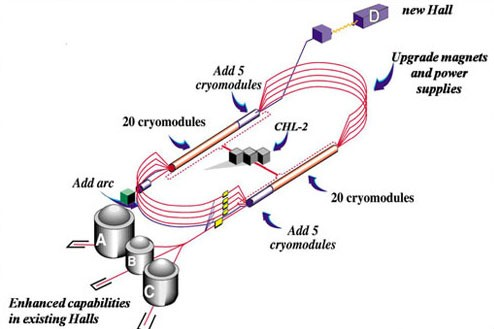
\includegraphics[width=0.5\textwidth]{images/cebaf.jpg}
    \caption{The Continuous Electron Beam Accelerator Facility.}
    \label{fig:cebaf}
\end{figure}
cavities were added to each of the linacs.  Four hall operation required the 
addition of a new 750 MHz RF separator, a new laser to the electron source and a
10th arc which allows delivery of the maximum beam energy to Hall D.  The 
upgrade allows CEBAF to accelerate electrons at a rate of 2.2 GeV per pass, up 
to 5.5 passes and currents upwards of 150 $\mu$A to all experimental halls.

%During the Spring of 2015, HPS was prepared to run at a beam energy of 2 GeV, 
%while the commissioning of the 750 MHz RF separator was taking place.  
%Unfortunately, the loss of one of the new CHLs caused the accelerator to 
%fallback to 6 GeV operation.  As a result, HPS instead ran with a beam energy of
%1.056 GeV.

\subsection{Electron Production and Injection}

The electrons injected into the accelerator were a result of photoemission from
a strained GaAs superlattice photocathode \cite{APL.2004.85.13}.  Each of the 
four experimental halls has a dedicated gain-switched fiber coupled laser of
wavelength 1560 nm.  The lasers are frequency doubled in order to produce light
of wavelength of 780 nm, matching the band gap of the superlattice cathode. The
lasers are phased shifted and are each pulsed for $\approx$ 40 ps at the 
frequency of 499 MHz.  Since the operational frequency of the accelerator 
cryomodules is 1497 MHz, four hall operation requires subharmonics of 499 MHz to
be chosen.  This is achieved by by ``cutting away'' pulses using an optical 
modulator \cite{kazimi2013source}.


The photoemission electrons are released into an extremely high vacuum
environment at a pressure of $10^{-11}$ to $10^{-12}$ Torr.  The free electrons
are then delivered into the injector by a 100 keV electron gun.  The injector
itself then accelerates the electron bunches to an energy of 67 MeV by 2 1/4
cryomodules before being delivered into the accelerator.

\subsection{Electron Acceleration}

% Need to add a sentence explain why we ran as a 6 GeV era detector
The CEBAF accelerator is composed of two linacs arranged in a racetrack
configuration as shown on Fig \ref{fig:cebaf}. Each of the linacs consist
of 25 cryomodules and are capable of accelerating the electron bunches 
by 2.2 GeV per pass up to a maximum of 5.5 passes per linac.  The number of 
passes depends on the energy requirements of the experiment taking place.
The electron bunches are delivered to Halls A, B and C by an RF separator
operating at a frequency of 499 MHz.  Delivery to Hall D uses an RF separator
of 750 MHz.

The acceleration of the electron beam takes place using a 5-cell 
superconducting radio frequency (SRF) cavities made of ultra-pure Niobium 
operating at 1497 MHz.  Two of the SRF cavities are joined and placed in a 
sealed helium container forming a cryounit.  Four cryounits are joined in an
insulating vacuum environment to form a cryomodule.  The cryomodules also
contain the necessary instrumentation both to power the SRF cavities and keep
them at an operating temperature of 2 K.

\section{Beam Line}

...

\section{Silicon Vertex Tracker}

\subsection{Layout}

The HPS SVT is comprised of six measurement layers, each consisting of a pair of
closely-spaced silicon planes as shown in Fig. \ref{fig:svt_layout_render}.
\begin{figure}[h]
    \centering
    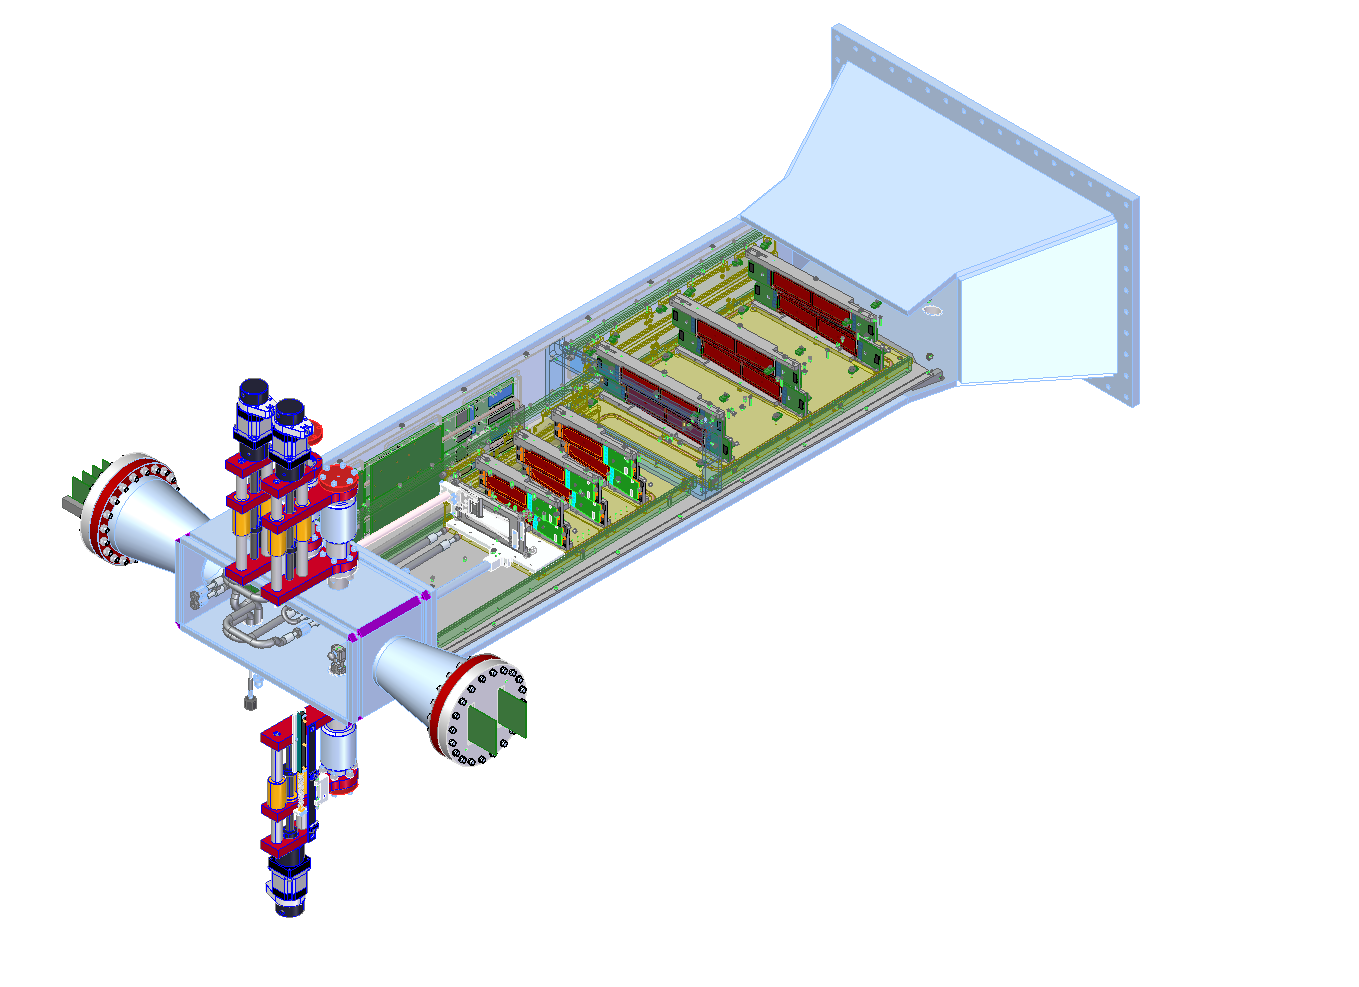
\includegraphics[width=0.9\textwidth]{images/svt_layout_render.png}
    \caption{A rendered view of the Silicon Vertex Tracker inside of the pair
             spectrometer vacuum chamber.}
    \label{fig:svt_layout_render}
\end{figure}
A stereo angle is introduced between the two planes within each layer allowing
for the measurement of both the vertical and bend coordinate of a hit, in turn, 
enabling full 3D hit reconstruction.  

The first three layers consist of a single sensor of coverage above and below
the beam plane and use a stereo angle of 100 mrad. In order to better match the
% needs a sentence explaining why 100 mrad stereo was used.  According to the
% proposal, it balances acceptance against vertexing resolution.
acceptance of the ECal, the coverage of the last three layers is two sensors 
% Insert a sentence explaining why 50 mrad? According to the proposal it's too
% cut down the number of bad tracks created from ghost hits due to layers with
% the same stereo angle.
% Why use a sixth layer? I guess it's not that important but should be in here
% nonetheless
wide and use a stereo angle of 50 mrad.  The choice of a 50 mrad angle for the
last three layers was meant to break the degeneracy that results in fake tracks
due to ghost hits in layers with the same stereo angle.  It must be noted that
only five layers are needed to match the full acceptance of the Ecal, however,
an improvement in the momentum resolution was observed with the addition of 
another layer.  In total, the SVT makes use of 36 sensors, which amounts to 
23,004 channels.

Since heavy photons are produced very forward, and the opening angle of it's 
decay products goes as $\sim m_{A}/E_{0}$, sensitivity to low mass $A'$ require
the tracker planes to be as close to the beam plane as possible.  When deciding
the distance of the first layer to the beam, several things  needed to be taken
into consideration including the amount of beam halo, the ability to resolve 
hits with pileup present and the ability to do pattern recognition in a high 
occupancy environment.  With all of this in mind, it was determined that the 
closest tolerable distance was 15 mrad, putting the active edge of layer 1 
at 0.5 mm from the beam center.  

The SVT layout is summarized in Table \ref{tab:svt_layout}.

%%%%%%%%%%%%%%%%%%%%%%%%%%%
%%% Table of SVT layout %%%
%%%%%%%%%%%%%%%%%%%%%%%%%%%
% I should use the survey positions here.
\begin{table}[t]
 \begin{center}
\begin{tabular}{l|cccccc}  
\hline
Layer & 1 & 2 & 3 & 4 & 5 & 6 \\ \hline
$z$ position from target (cm)    & 10 & 20 & 30 & 50 & 70 & 90 \\
Stereo angle (mrad) & 100 & 100 & 100 & 50 & 50 & 50 \\
Bend plane resolution ($\mu$m) & $\approx$6 & $\approx$6 & $\approx$6 & $\approx$6 & $\approx$6 & $\approx$6 \\
Non-bend plane resolution ($\mu$m) & $\approx60$ & $\approx60$ & $\approx60$ & $\approx120$ & $\approx120$ & $\approx120$ \\
Nominal dead zone in $y$ (mm) & $\pm$ 1.5 & $\pm$ 3.0 & $\pm$ 4.5 & $\pm$ 7.5 & $\pm$ 10.5 & $\pm$ 13.5 \\ 
\hline
\end{tabular}
\caption{The layout of the HPS SVT.}
\label{tab:svt_layout}
\end{center}
\end{table}
%%%%%%%%%%%%%%%%%%%%%%%%%%%

\subsection{Sensors}

At the energies at which HPS will operate, the uncertainty in both the mass and
vertex resolutions are dominated by multiple Coulomb scattering in the first 
few layers.  It was then empirical to choose a sensor technology that would 
reduce the material budget of the SVT in order to maximize the mass and vertex
resolutions.  Furthermore, the need to place the SVT in close proximity to the 
beam further required the sensors to be radiation tolerant.  Which these 
considerations in mind, a readily available batch of silicon microstrip sensors,
initially manufactured for the D0 Run IIb upgrade, were found satisfy all 
necessary requirements.

The sensors were manufactured by Hamamatsu Photonics Corporation on 
$\langle 100 \rangle$ crystal rotation silicon and are $p^{+}$ on $n$-bulk, 
single sided, AC-coupled and polysilicon-biased. The cut dimensions of the 
sensors are $100 \times 40.34$ mm$^{2}$ with an active area of 
$98.33 \times 38.34$ mm$^{2}$.  They are 320 $\mu$m thick and have a sense
(readout) pitch of 30 (60) $\mu$m. The sensor specifications are listed on 
Table \ref{tab:sensor_specs}.
\begin{table}[t]
    \centering
    \begin{tabular}{l|c}
        \hline
        Cut Dimensions & 100 mm x 40.34 mm \\
        Active Area & 98.33 mm x 38.34 mm \\
        Readout (Sense) pitch & 60 (30) $\mu$m \\
        \# Readout (Sense) strips & 639 (1277) \\
        Breakdown Voltage & $ > 1000$ V \\
        Total Interstrip Capacitance & $< 1.2$ pF/cm \\
        Defective Channels & $<1$ \% \\
        \hline
    \end{tabular}
    \caption{Specifications of the sensors used for the HPS SVT.}
    \label{tab:sensor_specs}
\end{table}

All sensors were qualified to 1000 V with only () out of () breaking down.  
During these test, leakage currents of less than 500 nA were observed.
IV curves for a subset of sensors can be seen on Fig. \ref{fig:sensor_iv_curves}.
The high breakdown voltage
\begin{figure}
    \centering
    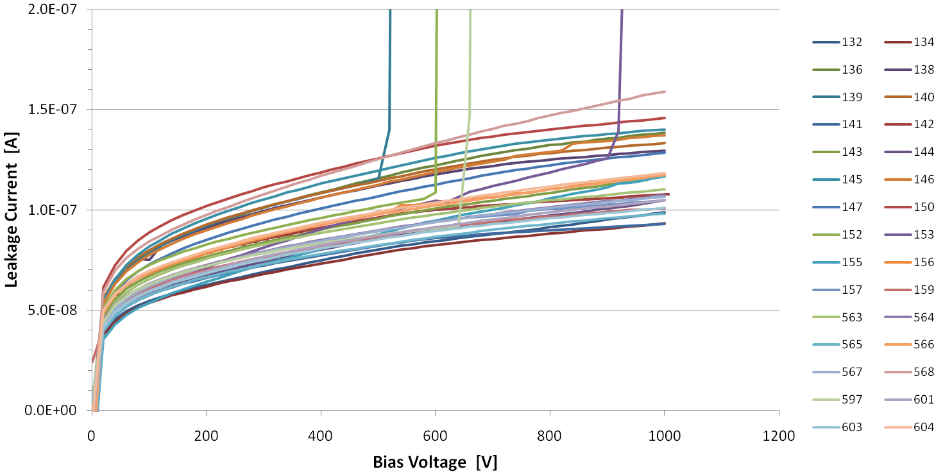
\includegraphics[width=0.9\textwidth]{images/sensor_iv_curves.png}
    \caption{IV curves for a subset of sensors used by HPS.}
    \label{fig:sensor_iv_curves}
\end{figure}
means that the sensors are capable of a dose tolerance of  1.5 
$\times 10^{14}$ 1 MeV neq/cm$^{2}$.  All sensors were determined to be fully 
depleted at $\approx$ 130 V. 

\subsection{Readout}

The sensors are continuously read out using the APV25 readout chip developed for
the Compact Muon Solenoid detector at the Large Hadron Collider 
\cite{apvdesign}. The APV25 has 128 channels, with each channel consisting
of a charge sensitive pre-amplifier coupled to CR-RC shaping amplifier and 192
cell deep analog pipeline.  A schematic of a single channel can be seen on 
Fig. \ref{fig:apv25_schem}.
\begin{figure}
    \centering
    \includegraphics[width=0.9\textwidth]{images/apv25_channel_schematic.png}
    \caption{A schematic of a single channel of the APV25 readout chip.}
    \label{fig:apv25_schem}
\end{figure}

The shaper signal is sampled at 40 MHz into the analog pipeline.  Only 160 cells
out of 192 are used to buffer the samples, the remaining being used to buffer
up to 10 triggers.  The 160 cell depth allows an external trigger decision of 
up to 4 $\mu$s.    

The APV25 can operate in two modes: peak mode and deconvolution mode.  In peak
mode, only a sample pipeline cell is read out corresponding to the maximum 
value of the CR-RC shape.  In deconvolution mode, three consecutive samples are
read out allowing for the reconstruction of the shaper output.

The analog pipeline is DC coupled to the Analog Pulse Shape Processor (APSP).

During the engineering run, the APV25's used the nominal  operating points with
a shaping time 50 ns.  The high occupancies expected during the engineering run
meant that overlapping of hits or ``pile-up'' were a concern.  In order to 
mitigate this problem, the APV25's were operated in deconvolution mode with
six consecutive samples readout per trigger.  The resulting signal shape 
observed during the engineering run is shown on Fig. \ref{fig:apv_shape}.  A 
\begin{figure}
    \centering
    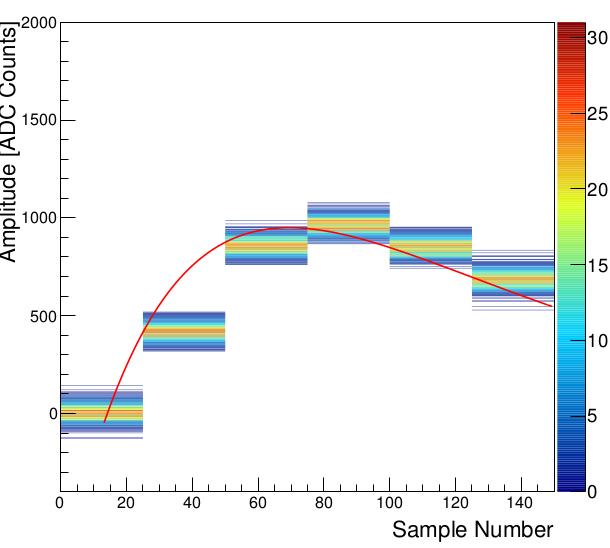
\includegraphics[width=0.9\textwidth]{images/sideB_response_ch535.png}
    \caption{The signal shape observed during the engineering run.}
    \label{fig:apv_shape}
\end{figure}
summary of the APV25 operating points used during the engineering run is listed
on Table \ref{tab:apv_specs}.
\begin{table}[t]
    \centering
    \begin{tabular}{l|c}
        \hline
        \hline
    \end{tabular}
    \caption{APV25 specs used during the engineering run.}
    \label{tab:apv_specs}
\end{table}

\subsection{Modules}

Each sensor requires 5 APV25 chips in order to readout all channels.  The 5 
APV25 chips are mounted on a FR4 electronic readout board, or hybrid, containing
filtering for the high voltage bias and a temperature sensor.  Since the pitch
of the APV25 and the sensors are similar, the chips were wirebonded directly to
the sensors without the need of a pitch adapter.

For layers 1-3 a ``half-module'' consist of a single sensor and hybrid glued 
onto a polyimide-laminated carbon fiber composite backing.  The half-modules 
for layers 4-6 consist of two sensors glued end onto the carbon fiber backing 
with hybrids on either side of them.  Due to space constraints, the hybrids used
by layers 4-6 have smaller footprint.  In order to further minimize the 
amount of material, a window is machined in the carbon fiber leaving the middle
of the sensor exposed. Fig. \ref{fig:l13_hm} and \ref{fig:l46_hm} show both a layer 1-3 and 4-6 
half-modules.
\begin{figure}
    \centering
    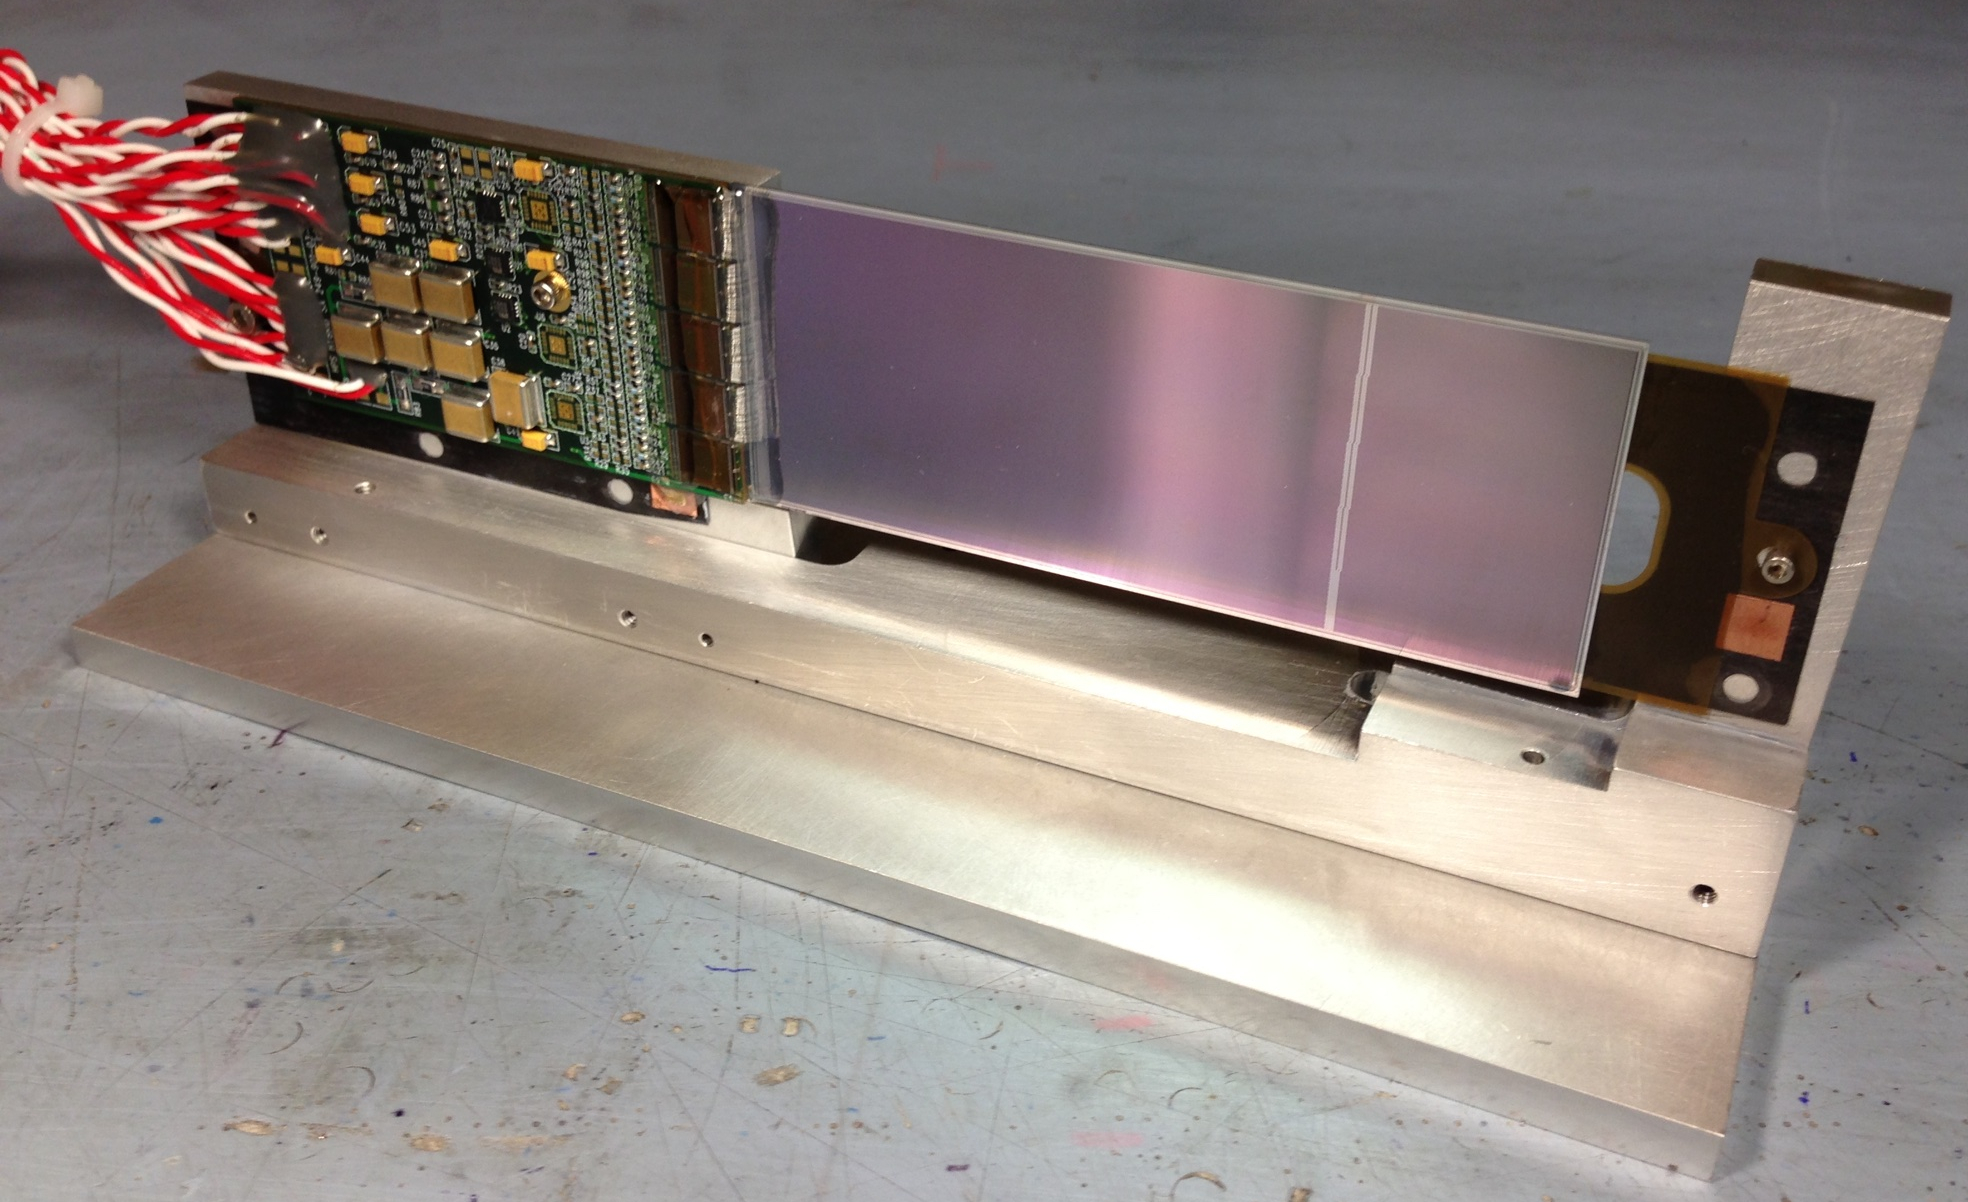
\includegraphics[width=0.9\textwidth]{images/l13_half_module.jpg}
    \caption{A layer 1-3 half-module used by the SVT. }
    \label{fig:l13_hm}
\end{figure}
\begin{figure}
    \centering
    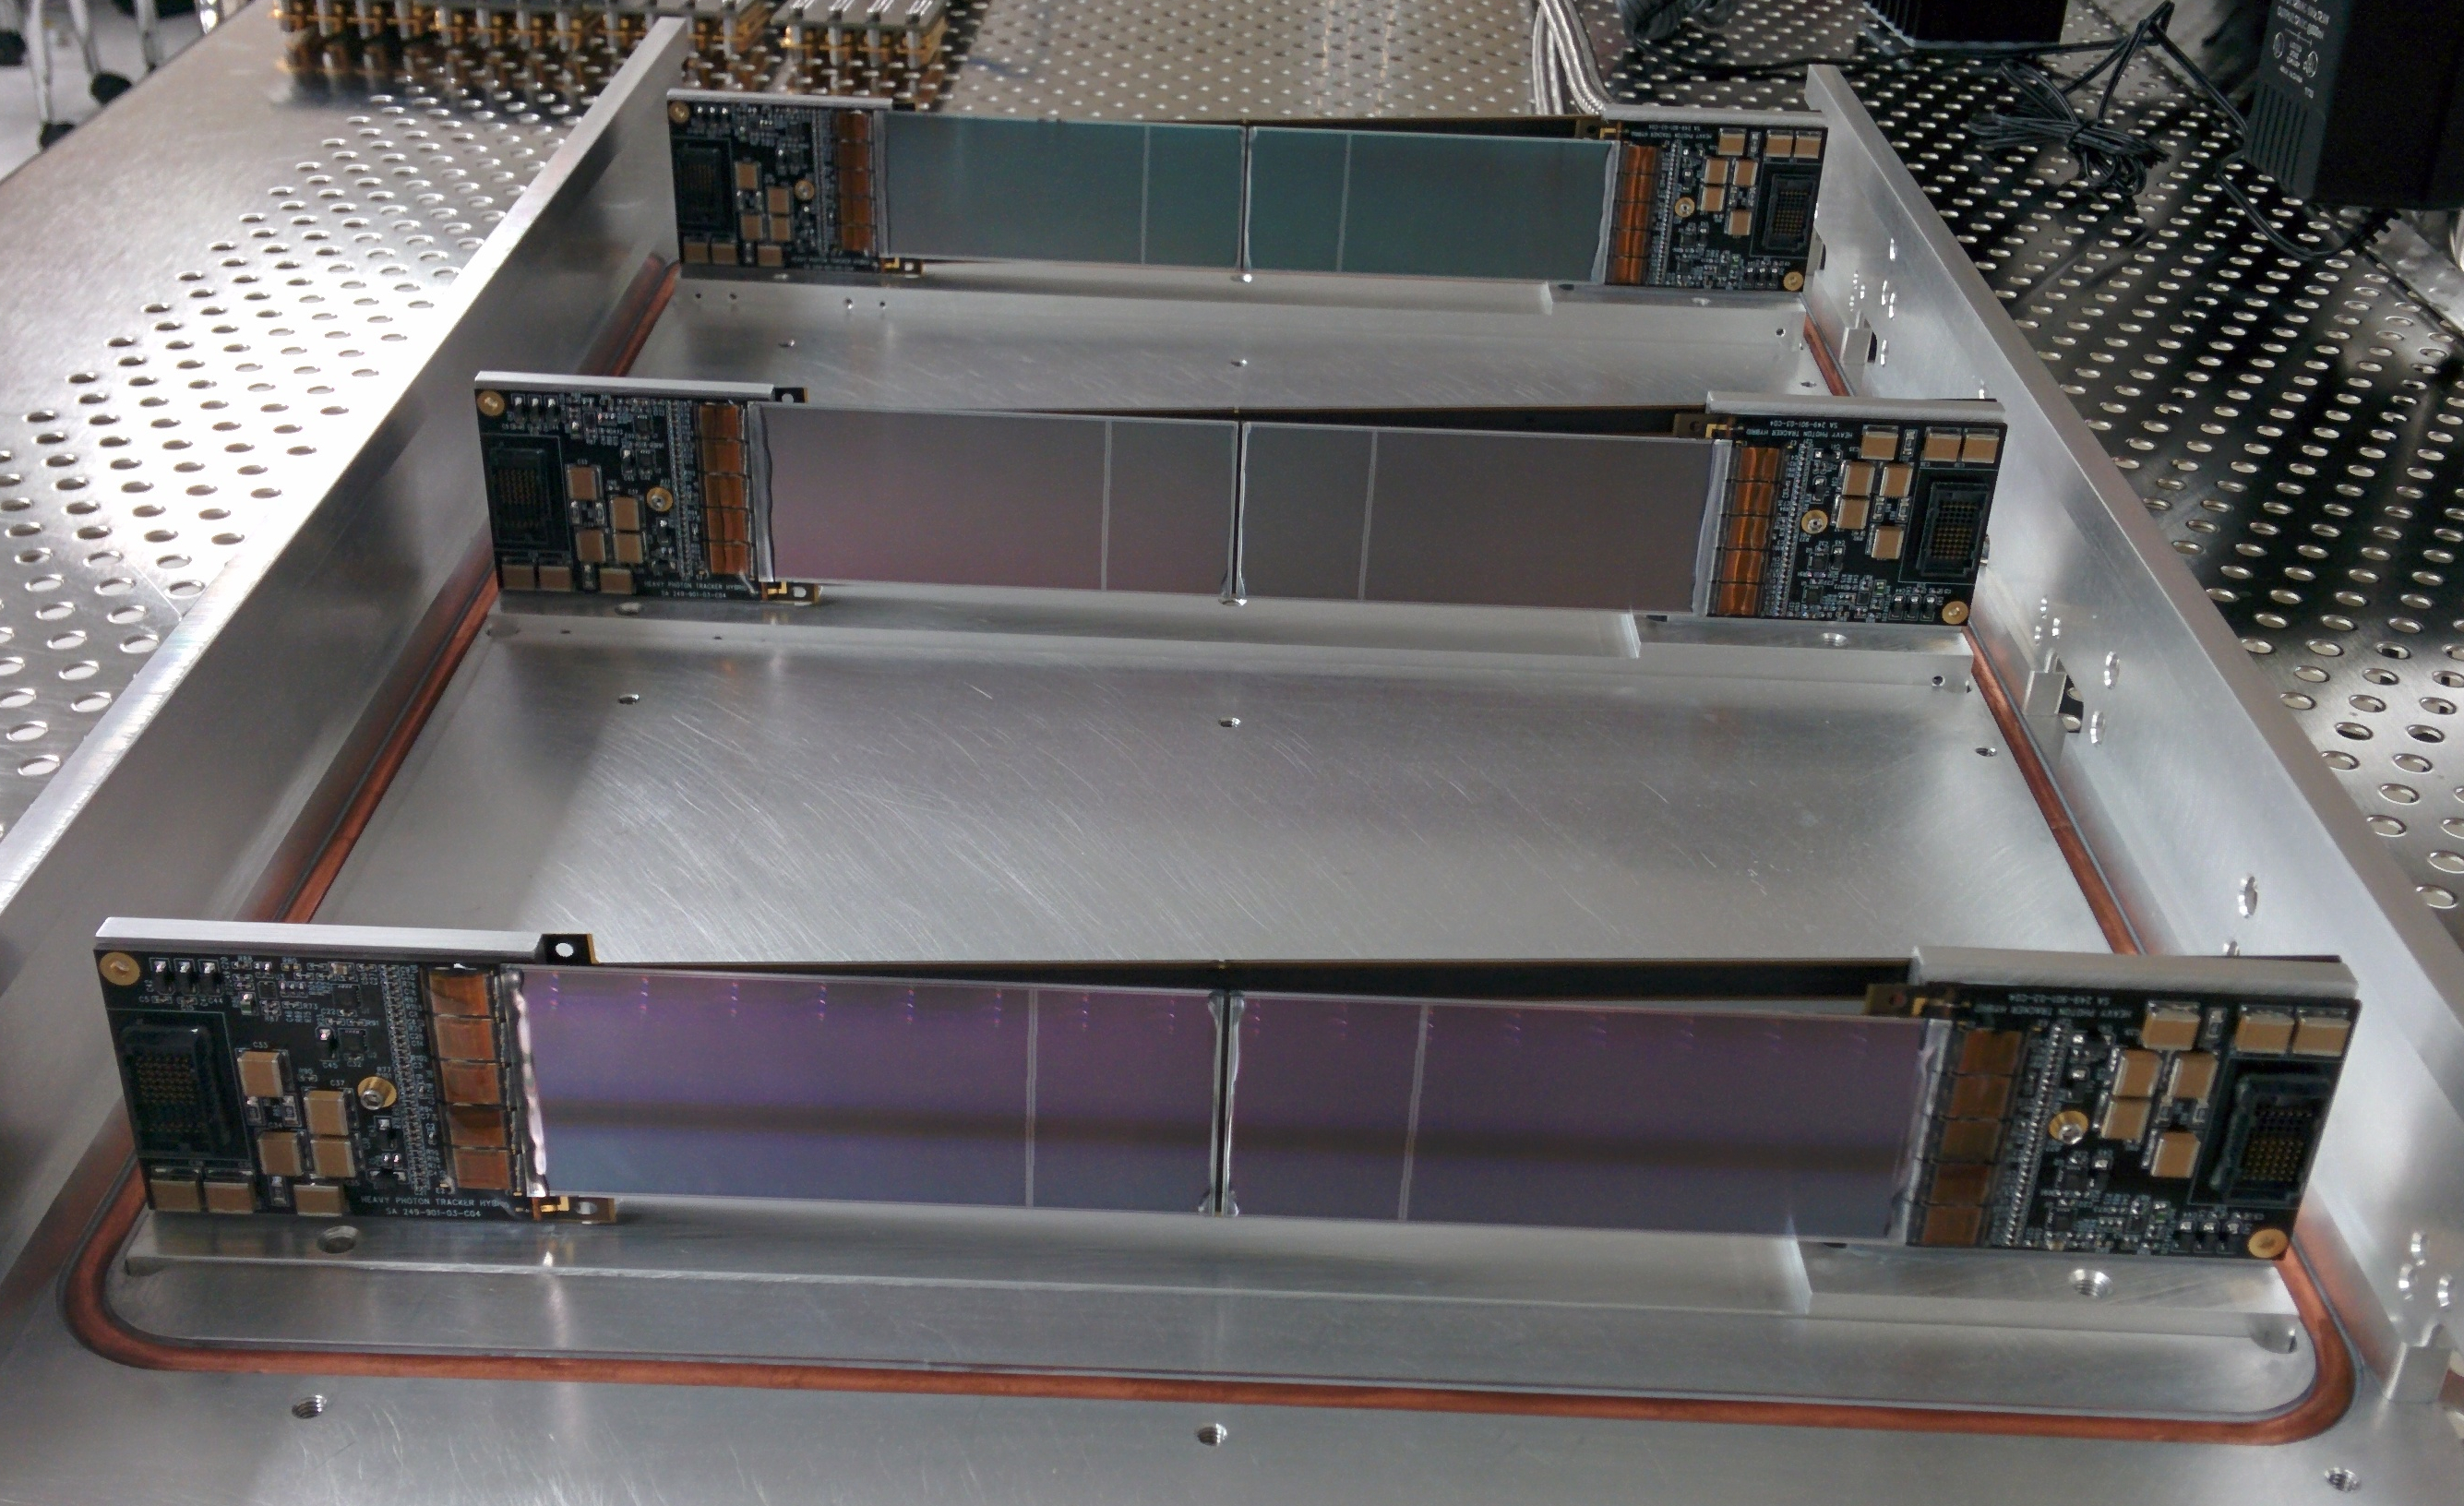
\includegraphics[width=0.9\textwidth]{images/l46_half_module.jpg}
    \caption{A layer 4-6 half-module used by the SVT. }
    \label{fig:l46_hm}
\end{figure}


\subsection{Mechanical Support, Cooling and Services}

...


\section{Electromagnetic Calorimeter}

The HPS Ecal is used as the primary trigger for the experiment as well as to
identify electrons and positrons.  It consist of two halves of lead-tungstate 
PbW0$_4$ crystals with each half mounted on an aluminum frame $\sim 137$ cm 
from the upstream edge of the analyzing magnet.  Each half is composed of five
layers of crystals with the four most outer layers consisting of 46 crystals and 
\begin{figure}
    \centering
    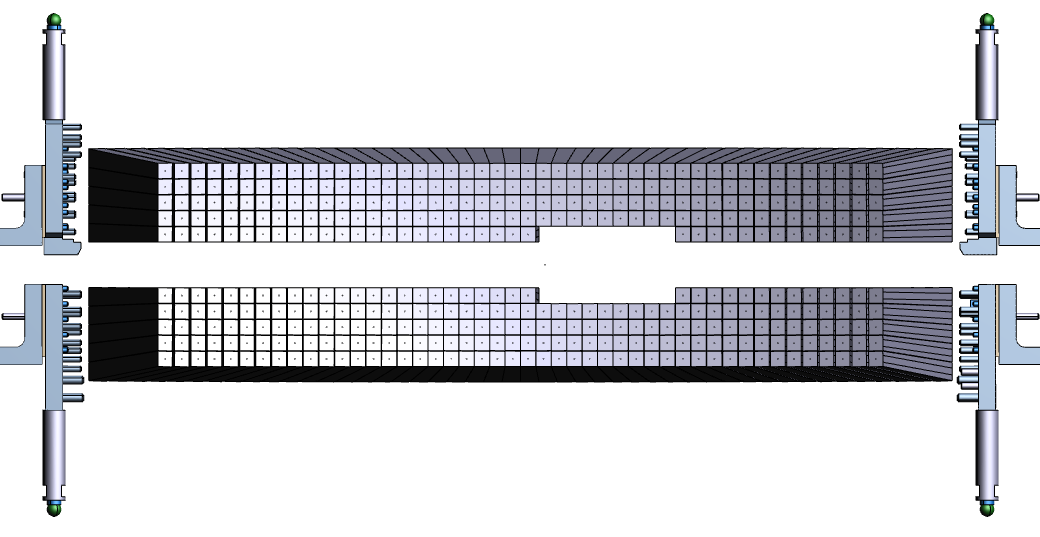
\includegraphics[width=0.8\textwidth]{images/ecal_layout.png}
    \caption{A rendering showing the arrangement of the Ecal crystals.  The Ecal
             is split into upper and lower modules in order to accommodate the 
             ``dead zone''.  The crystals removed from the first layer allow
             a larger opening for the outgoing electron and photon beams.}
    \label{fig:ecal_layout}
\end{figure}
the layer closest to the beam plane consisting of 37. The removal of the 9 
crystals from the inner layer was necessary to allow the outgoing electron and
photon beams to pass through unimpeded.  Each half is enclosed in a temperature
controlled environment held at 1$^{\circ}$ F which encroaches on the Ecal 
vacuum chamber.

Each of the crystals is 16 cm long and trapezoidal in shape with a front face
dimension of $1.3 \times 1.3$ cm$^2$ and a back face dimension of $1.6 \times
1.6$ cm$^2$.  In order to maximize the light yield, the crystals were wrapped
in VM2000 non-metallic reflector film. A Hamamatsu S8664-1010 Avalanche 
Photodiode (APD) with a photosensitive area of $10 \times 10$ mm$^2$ was glued
to the back of each crystal and used to read out the signals collected by the
crystals.  
\begin{figure}
    \centering
    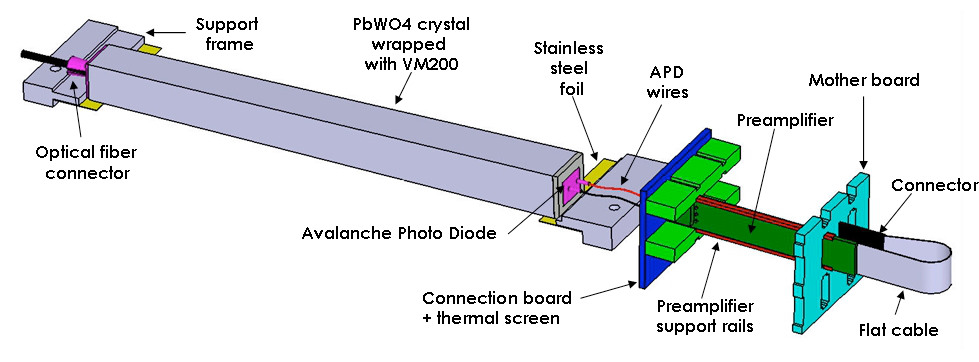
\includegraphics[width=0.8\textwidth]{images/ecal_crystal.png}
    \caption{Rendered view of an HPS Ecal module consisting of a 16 cm PbW$_4$
             crystal, Avalanche Photodiode and preamplifier board.}
    \label{fig:ecal_crystal}
\end{figure}

%\section{Trigger and Data Acquisition}
 
%\subsection{SVT DAQ}


%The low voltage differential signals (LVDS) from each of the APV25's are 
%transferred via twisted pair wires to a FEB to undergo digitization
%and further processing.  At the FEB, the LVDS signal is first amplified to match
%the dynamic range of the 14 bit analog to digital converter (ADC). The ADC 
%samples the signal at 41.667 MHz and digitizes it to a value between 0 and 
%16384.  The digitized signals are then transferred to () field programmable gate
%arrays (FPGA) where thresholds are applied. If a signal is found to have three
%samples above 3 noise RMS above baseline.

 %Thresholds are derived from baseline runs and were set to be 3 sigma noise RMS
 %above baseline.

% Those signals which pass the threshold requirement are transferred through 
% mini SAS wires to a board on the vacuum  where they undergo optical conversion.
%The optical signal is then transferred over ~10 m fibers to the ATCA crate.


%\subsection{Ecal DAQ}

 % Maybe show an example of how the signal looks emerging from the APV?


